\chapter{Searching Algorithms}

In this chapter we will look into some algorithms that search for a specific integer\footnote{The algorithms also work for other data types. However integer is selected for easier understanding.} in an array, and return its index in the array. We will look at how they work and analyze their efficiency (using time complexity). We will only focus on implementation using arrays.

\section{Further resources (Ch 7-8)}

Watching animations of these algorithms is useful in understanding how they work. I don't have a specific YouTube channel in mind. Yet algorithms in this and the next chapter are all very famous, I am sure you can find plenty of videos about them online.

\section{Linear search}

Linear search simply searches through the array from left to right, scanning the elements one by one until a match is found. Linear search returns \textit{n} if the integer is not found.\footnote{The choice of $n$ is helpful in making code for \texttt{linearSearch3} and the final \texttt{linearSearch} concise. We could make it return anything by adding more code at the end if required.}

\begin{lstlisting}
int main(){
    int x[] = {3,1,4,1,5,9,2,6};

    cout << linearSearch(x,8,4) << endl; //2
    cout << linearSearch(x,8,2) << endl; //6
    cout << linearSearch(x,8,7) << endl; //8 (not found, return n)
}
\end{lstlisting}

If we just want to know if the element is in the array, we can check it by \texttt{i$<$n}:

\begin{lstlisting}
int i = linearSearch(x,8,target);
if(i<n)
    cout << target << " found at location " << i << endl;
else 
    cout << target << " not found" << endl;
\end{lstlisting}

Now, after we have clarified what it does, let's implement it in C++.
\vspace{6mm}

C++: \textit{(NOT the one you should follow)}
\begin{lstlisting}
int linearSearch1(int x[], int n, int target){
    int i = 0;
    int found = n; //found is n exactly when the target is not found, or it stores the index where the element is found
    while(i<n){
        if(x[i]==target) found = i;
        i++;
    }
    return found;
}
\end{lstlisting}

\textit{Exercise: Determine the behaviour of \texttt{linearSearch1} when there are duplicates in the array.}
\vspace{6mm}

\texttt{linearSearch1} runs in $O(n)$ time because the while loop is run $n$ times and each iteration takes constant time. It is not ideal because the loop continues even when a match is found, better versions quit the loop when a match is found, either with the help of the variable \texttt{found}, with a \texttt{break} statement, or simply returning early.
\vspace{6mm}

C++: (Using a variable)
\begin{lstlisting}
int linearSearch2(int x[], int n, int target){
    int i = 0;
    int found = n; //found is n exactly when the target is not found, or it stores the index where the element is found
    while(found != n && i<n){
        if(x[i]==target) found = i;
        i++;
    }
    return found;
}
\end{lstlisting}

C++: (Using \texttt{break})
\begin{lstlisting}
int linearSearch3(int x[], int n, int target){
    int i = 0;
    while(i<n){
        if(x[i]==target) break;
        i++;
    }
    return i;
}
\end{lstlisting}

C++: (returning early)
\begin{lstlisting}
int linearSearch4(int x[], int n, int target){
    int i = 0;
    while(i<n){
        if(x[i]==target) return i;
        i++;
    }
    return i; //not found
}
\end{lstlisting}

If you want to eliminate the need of any of those, you could write the loop in a more compact format, giving the best linear search code in my opinion.
\vspace{6mm}

C++: \textit{(Exercise:  Try to re-implement yourself.)}
\begin{lstlisting} 
int linearSearch(int x[], int n, int target){
    int i = 0;
    while(i<n&&x[i]!=target) i++;
    return i;
}
\end{lstlisting}

\textit{Exercise: Determine the behaviour of \texttt{linearSearch2,3,4} and \texttt{linearSearch} when there are duplicates in the array.}

\vspace{6mm}

\textit{Exercise: Can we change the order of the tests of the while loop for \texttt{linearSearch2}? How about \texttt{linearSearch}?}
\vspace{6mm}

The worst case of \texttt{linearSearch2,3,4} and \texttt{linearSearch} occurs when the target is not found or the target is the last element, the while loop is run \textit{n} times to search through the whole array before returning. Therefore the worst case time complexity is still $O(n)$.
\footnote{This part of the notes follows the pattern in \cite{ip:stringsearching}}
% \footnote{Reference: Grau, B. C., Pitt-Francis, J., Spivey, M., \& Lowe, G. (2023). \textit{Example: string searching}. Imperative Programming Parts 1 and 2.}

\if\invariant1

\subsection*{Invariant}

We can write an invariant for \texttt{linearSearch}.

\begin{center}
    \textit{\textbf{Invariant:}\hspace{6mm} target is not found in $A[0..i)$}
\end{center}

We will show that maintain this invariant from start to finish. 
\vspace{6mm}

\textbf{Initialisation:} Initially, we set i=0. A[0..0) is equal to an empty array. As anything cannot be found inside an empty array, invariant holds trivially.
\vspace{6mm}

\textbf{Maintenance:} The loop carries on meaning that $x[i]$ is not the target, we can easily extend our invariant so that it is now target is not found in $A[0..i+1)$ i.e. target is not found in $A[0.._{new}i)$
\vspace{6mm}

\textbf{Termination:} Termination is non-trivial, we have to separate our discussion into two cases, depending on which condition no longer holds leading to the termination of the loop.

\textit{Case 1:} $i=n$, by the invariant, target is not found in $A[0..n)$, meaning that the target is not found in the whole array, we should return $n$ by the specification of linear search, which is inline with what we are returning.

\textit{Case 2:} target $ = x[i]$. Target is found! But before we are too thrilled and decided to return $i$ immediately, we need to think twice whether $x[i]$ is the leftmost occurrence of the target. Luckily, our invariant tells us that the target is not found in $A[0..i)$, reassuring us that $A[i]$ is indeed the leftmost occurance of the target.\footnote{Cited from \cite{ip:inv}}
% \footnote{Reference: Grau, B. C., Pitt-Francis, J., Spivey, M., \& Lowe, G. (2023). \textit{Invariants}. Imperative Programming Parts 1 and 2.}

\fi
\pagebreak

\section{Binary search}

In fact, we can do better. Yet this requires the array to be \textbf{sorted} beforehand.

The idea is, we compare the target with the middle element of the array, say \texttt{x[m]}, and we shrink the array in half because we know the element can never be in one of the halves of the array. A detailed explanation of why is as follows:
% Every time we can cut the array in half, and compare the target with the middle element (x[m]). 
\vspace{6mm}

Let's say the segment that the target might be in is x[i..j) (including i and excluding j). We try to maintain that structure that the right hand index is always excluded, and the left hand index is always included, to avoid complications of code.
\vspace{6mm}

If x[m] $<$ target, we know all elements with index $<=$ m are also smaller than the target, because the array is sorted. We can set the lower boundary (i) to m+1.

If x[m] $>$ target, we know all elements with index $>=$ m are also larger than the target, because the array is sorted. We can then set the upper boundary (j) to m. (excluding m)
\vspace{6mm}

In either case, around half of the array is eliminated from consideration.

Process continues until the target is found (x[m] = target).
\vspace{3mm}

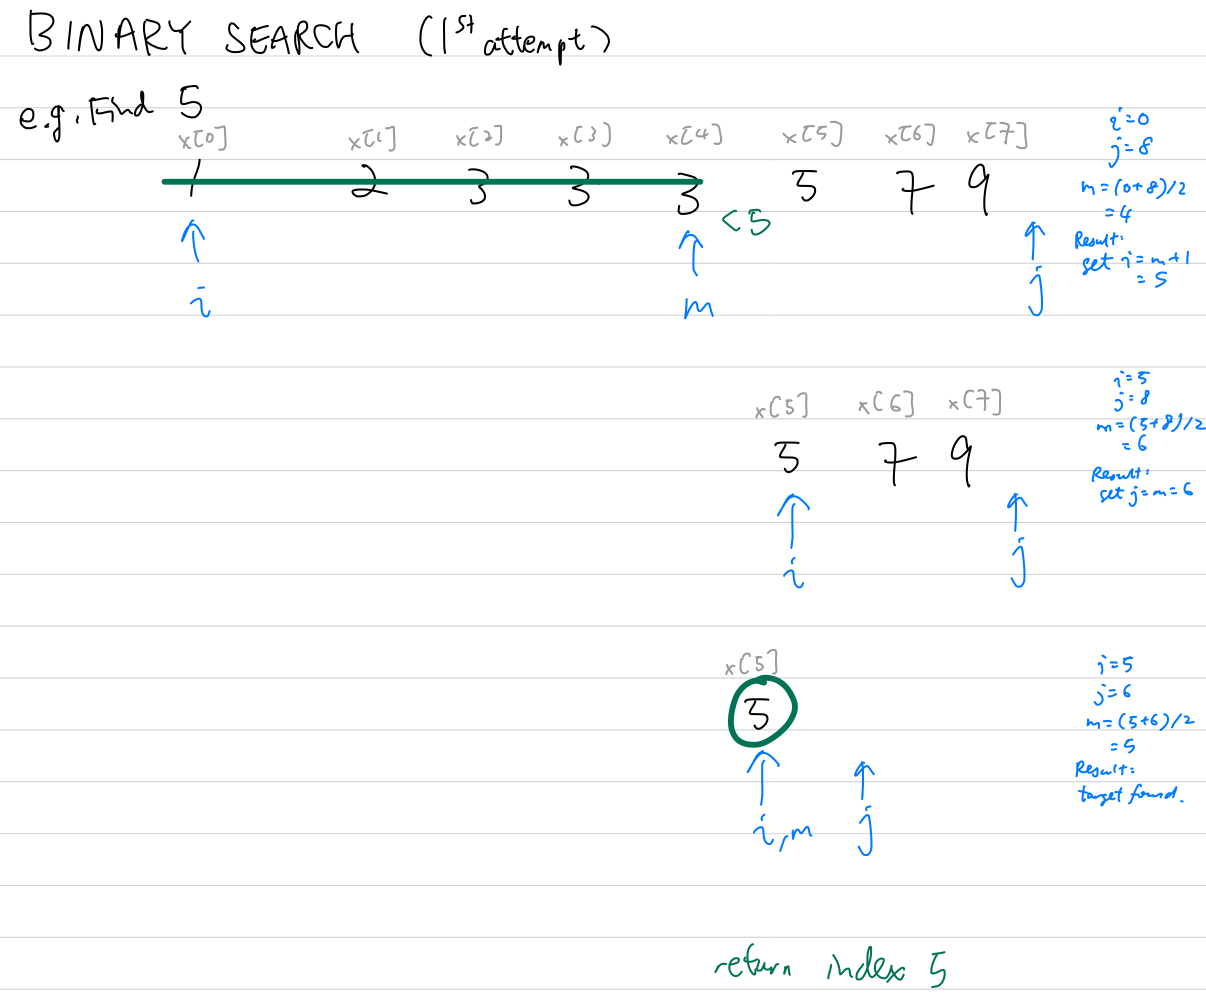
\includegraphics[width=12cm]{images/ch7-binarysearch1.png}
\pagebreak

Here is my first attempt in writing the binary search code: \textit{(NOT the one you should follow)}

\begin{lstlisting}
int binarySearch1(int x[], int n, int target){
    int i=0;
    int j=n;
    while(i<j){
        //array segment: x[i..j)
        //stopping condition is i=j because the array would be empty
        int m = (i+j)/2; //rounded down automatically by C++
        if(x[m]<target){
            //new array segment: x[m+1..j)
            i = m+1;
        }else if(x[m]>target){
            //new array segment: x[i..m)
            j = m;
        }else{
            //a match is found
            return m;
        }
    }
    return -1; //not found
}

int main(){
    int x[] = {1,2,3,3,3,5,7,9};
 
    cout << binarySearch1(x,8,1) << endl; //0
    cout << binarySearch1(x,8,5) << endl; //5
    cout << binarySearch1(x,8,7) << endl; //6

    //there are multiple 3s, should it return 2,3 or 4? Is the behaviour consistent?
    cout << binarySearch1(x,8,3) << endl; //4

    //8 is not in the array, can it return something more meaningful other than -1?
    cout << binarySearch1(x,8,8) << endl; //-1
}
\end{lstlisting}

\pagebreak

\subsection*{To be precise}

\textit{Difficult topic}
\vspace{6mm}

\texttt{binarySearch1} seems to be working nicely most of the time except in the last two examples. In fact, they are \textbf{edge cases} that require special attention. 

\begin{itemize}
    \item Duplicate targets in the array: To maintain consistency, we should return the location of the leftmost occurrence of the target. Hence, we cannot just stop when a match is found.
    \item Targets that are not found in the array: We should return the location where the target can be inserted to maintain the order of the array. 
\end{itemize}

% How about duplicate targets in the array? To maintain consistency, we should return the location of the leftmost occurrence of the target. Hence, we cannot just stop when a match is found.

% How about targets that are not found in the array? We should return the location where the target can be inserted to maintain the order of the array. 

The moral is to consider the edge cases before writing any code, as we need to change our whole concept slightly to cater these edge cases. (Surprisingly these changes lead to neater code)
\vspace{6mm}

We will imagine that we split the array into three sections, x[0..i) contains all elements that are checked $<$ target, x[i..j) contains all elements that are not checked yet, and x[j..n) contains all elements that are checked $>=$ target. We will maintain this relationship from start to finish. 

Initially, we set i=0, j=n, so that the first and the last sections are empty, signifying all elements are unchecked. Then we gradually check the elements using binary search (similar to the concept explained in the previous section), until i=j, meaning that all elements are checked. Then we return a value.
\vspace{6mm}

Which value shall we return? x[0..i) contains all elements that $<$ target, and x[i..n)\footnote{remember i=j when binary search terminates} contains all elements that $>=$ target. 

If the target is present, it will be at location i. If there are duplicates, the leftmost occurrence will be at location i. If the target is not present. The proper location to insert it is also location i. So i is the correct value to return in all cases. Neat!
\vspace{6mm}

Followed are some illustrations that further elaborate on the concept, and also the implementation in C++.
\vspace{6mm}

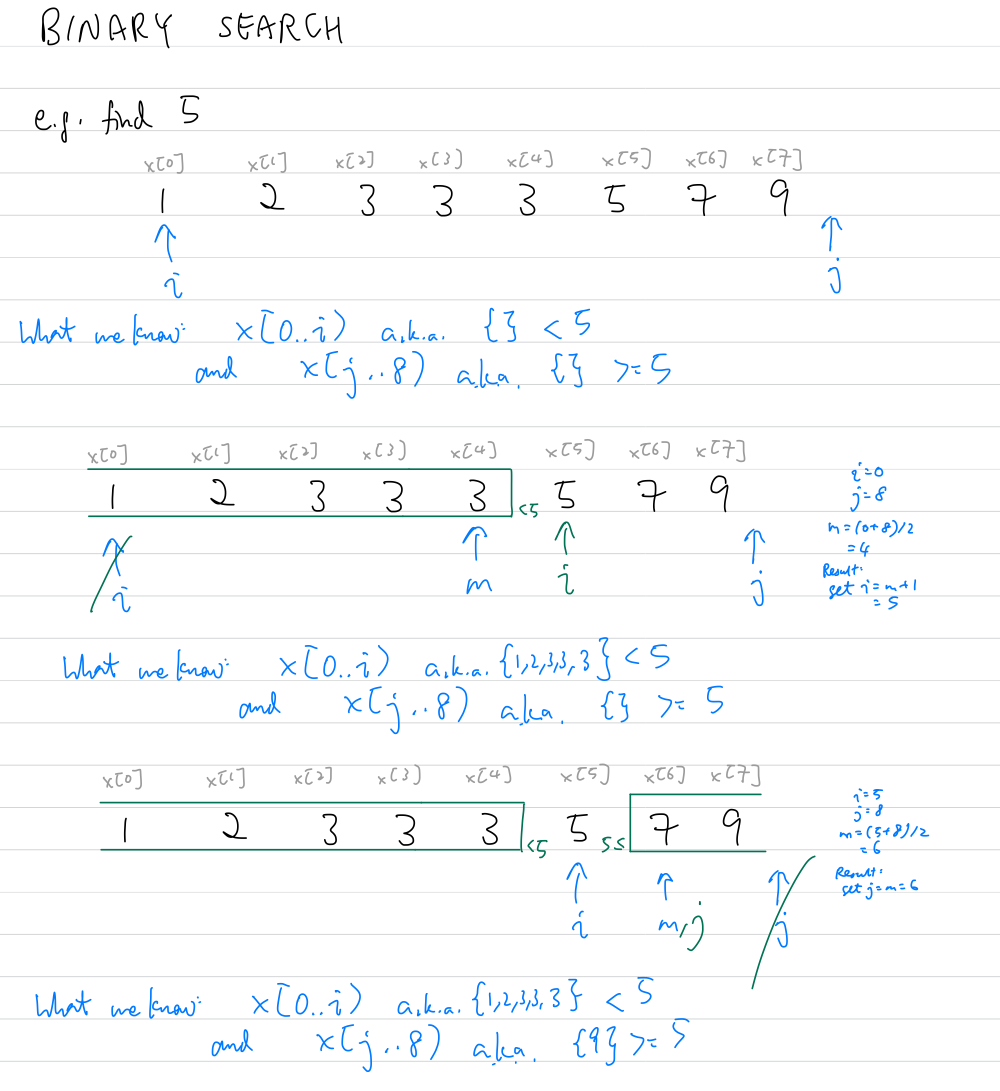
\includegraphics[width=14cm]{images/ch7-binarysearch51.png}

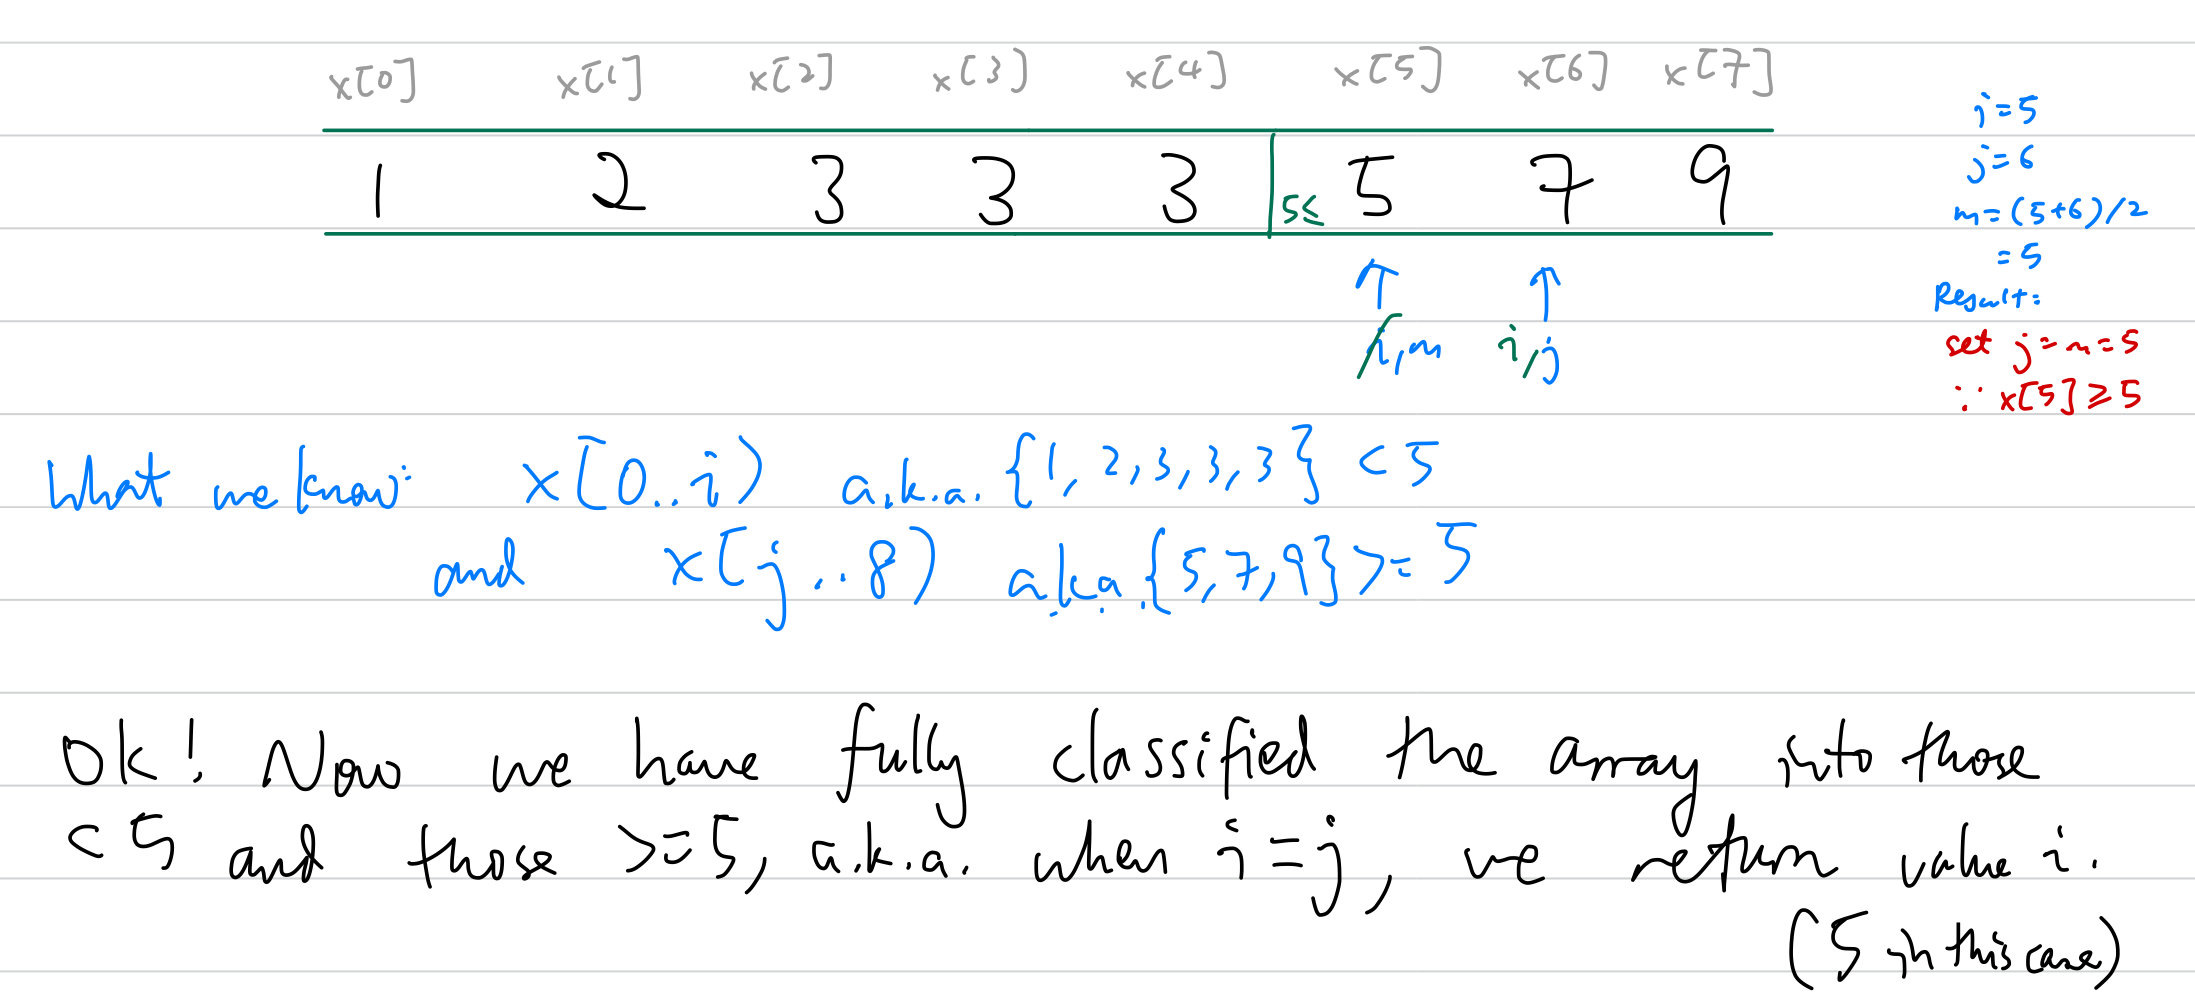
\includegraphics[width=14cm]{images/ch7-binarysearch52.png}

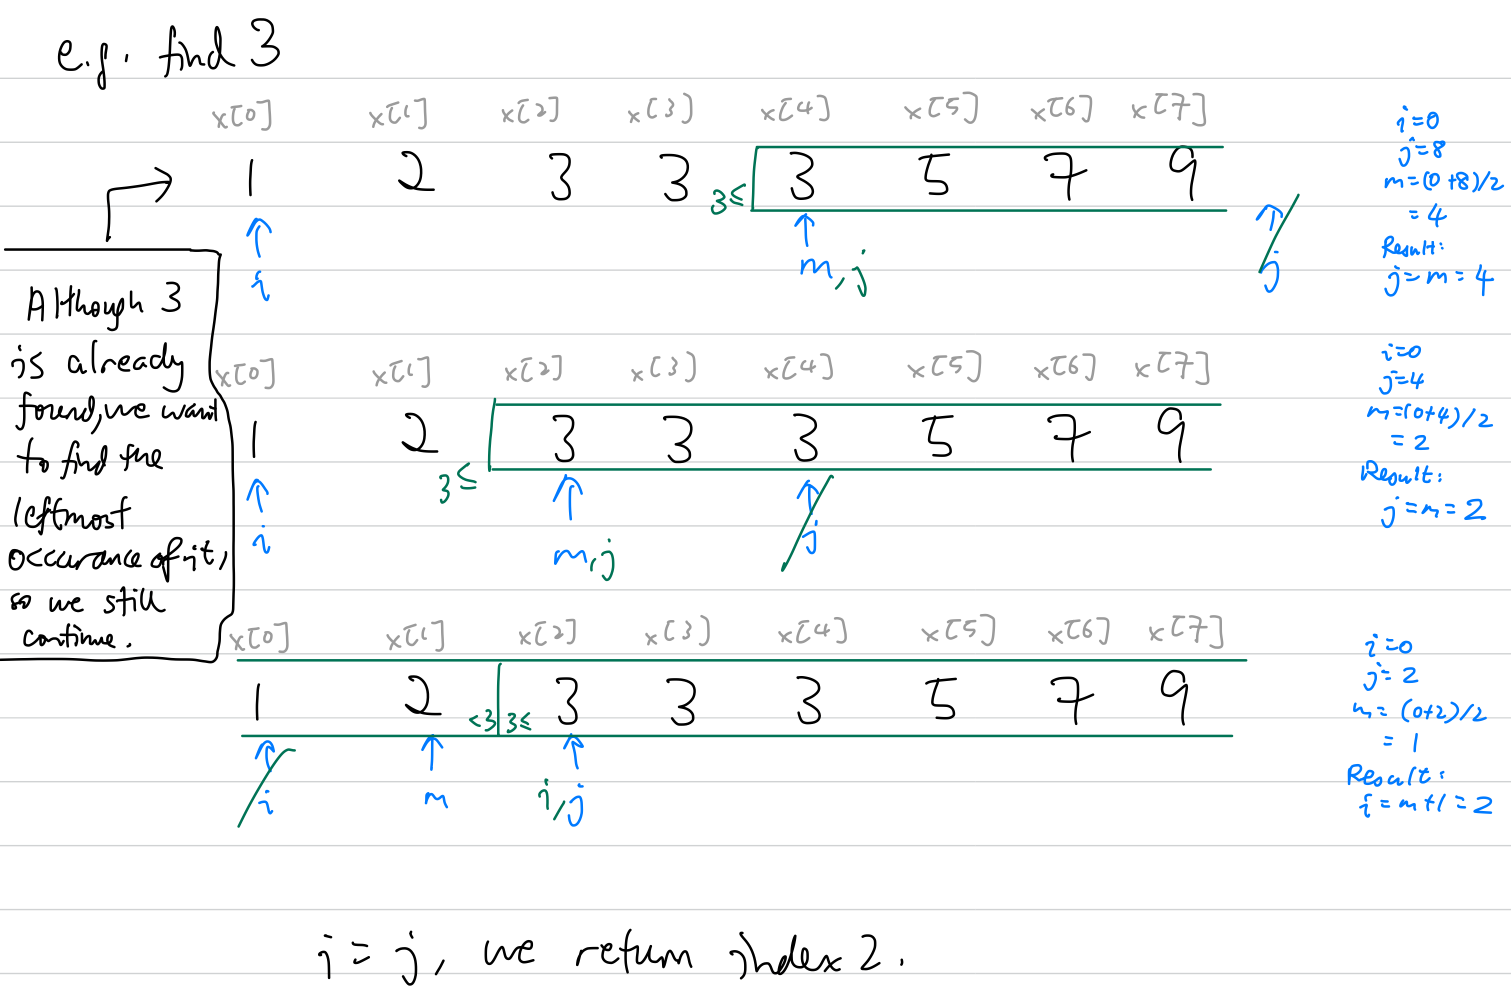
\includegraphics[width=14cm]{images/ch7-binarysearch3.png}

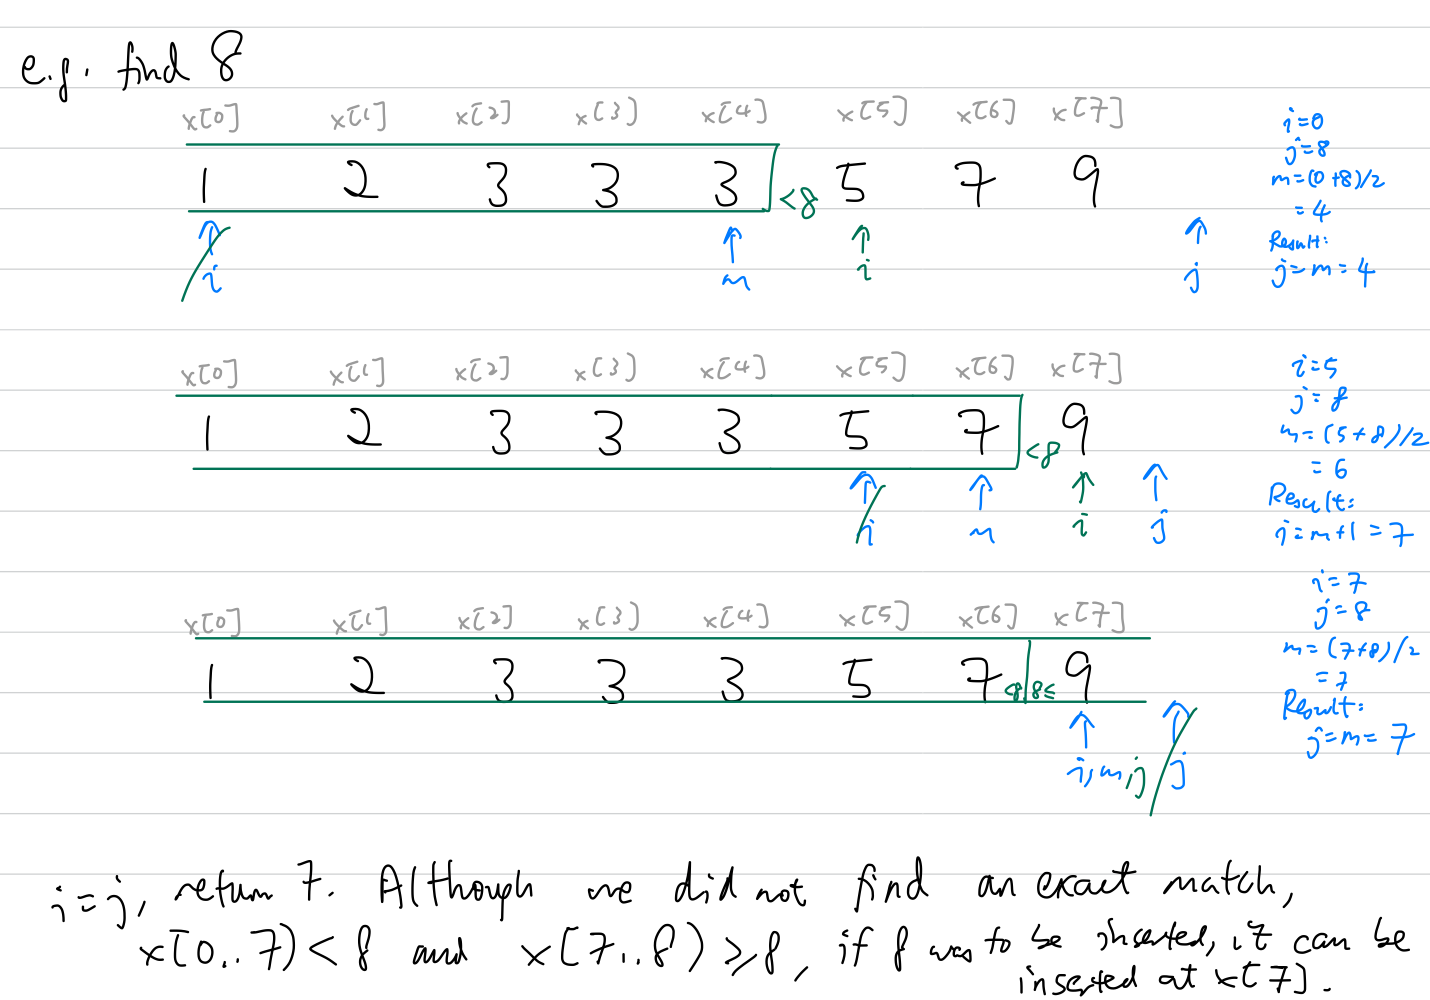
\includegraphics[width=14cm]{images/ch7-binarysearch8.png}

\pagebreak

C++: \textit{(Exercise:  Try to re-implement yourself.)}\footnote{Cited from: \cite{ip:binsearch}}

\begin{lstlisting}
int binarySearch(int x[], int n, int target){
    int i=0;
    int j=n;
    while(i<j){
        //array segment: x[i..j)
        int m = (i+j)/2;
        if(x[m]<target){
            //new array segment: x[m+1..j)
            i = m+1;
        }else {
            //new array segment: x[i..m)
            j = m;
        }
    }
    return i;
}

int main(){
    int x[] = {1,2,3,3,3,5,7,9};

    cout << binarySearch(x,8,1) << endl; //0
    cout << binarySearch(x,8,5) << endl; //5
    cout << binarySearch(x,8,7) << endl; //6

    cout << binarySearch(x,8,3) << endl; //2 (leftmost occurance)

    cout << binarySearch(x,8,8) << endl; //7 (the index that number 8 should be inserted)
}
\end{lstlisting}

If we just want to know if the element is in the array, we could easily check by \texttt{i$<$n \&\& x[i]==target}:

\begin{lstlisting}
int i = binarySearch(x,8,target);
if(i<n && x[i]==target)
    cout << target << " found at location " << i << endl;
else 
    cout << target << " not found, it can be inserted at location " << i << endl;
\end{lstlisting}

\textit{Exercise: Is \texttt{i<n} necessary? Can we change the order of the tests?}
\vspace{6mm}

Time complexity: $O(\log n)$ comparisons
\vspace{6mm}

In each step, around half of the array is eliminated from consideration, giving a total of $\log_2 n$ steps. Each step takes constant time.

\if\invariant1

\subsection*{Invariant}

It is a good idea to use invariants to proof that our binary search code is correct, and there are no off by one errors. The reasoning is actually very similar to what we had above, but we will make it formal in this section. First, we establish the invariant based on the "three sections" concept we had: 

\begin{center}
    \textit{\textbf{Invariant:}\hspace{6mm} x[0..i) $<$ target and x[j..n) $>=$ target}
\end{center}

We will show that maintain this invariant from start to finish. 
\vspace{6mm}

\textbf{Initialisation:} Initially, we set i=0, j=n, so that the first and the last sections are empty, hence satisfying the invariant trivially. It also represents that all elements are unchecked. Then we gradually check the elements.
\vspace{6mm}

\textbf{Maintenance:} Let's say the segment unchecked is x[i..j) (including i and excluding j). We try to maintain that structure that the right hand index is always excluded, and the left hand index is always included, to avoid complications of code. We will analyse the loop body based on which part of the if statement is taken.

\textit{Case 1:} If x[m] $<$ target, we know all elements with index $<=$ m are also smaller than the target, because the array is sorted. We can set the lower boundary (i) to m+1 (including m+1) with the invariant still maintained.

\textit{Case 2:} If x[m] $>=$ target, we know all elements with index $>=$ m are also larger than the target, because the array is sorted. We can then set the upper boundary (j) to m (excluding m) with the invariant still maintained.
\vspace{6mm}

\textbf{Termination:} We stop when i=j, meaning that all elements are checked. Then we return a value. x[0..i) contains all elements that $<$ target, and x[i..n)\footnote{remember i=j when binary search terminates} contains all elements that $>=$ target by the invariant. 

If the target is present, the return value should be at location i. If there are duplicates, the leftmost occurrence will be at location i. If the target is not present. The proper location to insert it is also location i. So i is the correct value to return in all cases. Neat!\footnote{Cited from: \cite{ip:binsearch}}

% \footnote{Reference: Grau, B. C., Pitt-Francis, J., Spivey, M., \& Lowe, G. (2023). \textit{Binary Search}. Imperative Programming Parts 1 and 2.}
\vspace{6mm}

\fi

\section{Conclusion}

\begin{table}[h]
    \centering
    \begin{tabular}{|m{6em}|m{9em}|m{18em}|}
        \hline  
        \textbf{Searching Algorithms} & 
        \multicolumn{2}{l|}{Goal: Find location of a target in an array}
        \\ \hline \hline
        
        Algorithm &
        Time Complexity & 
        Remarks
        \\ \hline \hline
        
        Linear search &
        $O(n)$ &
        Works for all arrays
        \\ \hline
        
        Binary search &
        $O(\log n)$ &
        Works only for sorted arrays, much faster
        \\ \hline
    \end{tabular}
\end{table}

Binary search should be used when the data is sorted (which is commonly the case), linear search otherwise.